\documentclass[12pt]{article}

\usepackage{amsmath,amssymb,amsthm,enumerate,graphicx}
\usepackage{ifthen,latexsym,syntonly}
\usepackage{setspace}
\usepackage{mathabx}
%\usepackage[showrefs]{refcheck}  %use this to show equation and section labels
\usepackage{color}
\usepackage[round,comma,authoryear]{natbib}   % for natbib
%\usepackage{subfigure}
 %\usepackage{graphics}
\usepackage{float}
\usepackage{epstopdf}
\usepackage{mathabx}
\bibliographystyle{mynat}

\onehalfspacing



\setlength{\textwidth}{6.5in}
\setlength{\textheight}{8.5in}
\usepackage{color}
\allowdisplaybreaks[3]
\usepackage{calc,xspace}
\definecolor{wacky}{rgb}{1,0,1}
\onehalfspacing

\newcommand{\wacky}[1]{{\large\textcolor{wacky}{#1}} }

\definecolor{ForestGreen}{RGB}{34, 139, 34}


\newtheorem{theorem}{Theorem}[section]
\newtheorem{remark}[theorem]{Remark}
\newtheorem{assumption}[theorem]{Assumption}
\newtheorem{case}[theorem]{Case}
\newtheorem{claim}[theorem]{Claim}
\newtheorem{corollary}[theorem]{Corollary}
\newtheorem{condition}[theorem]{Condition}
\newtheorem{criterion}[theorem]{Criterion}
\newtheorem{definition}[theorem]{Definition}
\newtheorem{example}[theorem]{Example}
\newtheorem{lemma}[theorem]{Lemma}
\newtheorem{problem}[theorem]{Problem}
\newtheorem{proposition}[theorem]{Proposition}
\newtheorem{thm}[theorem]{Theorem}
\providecommand{\keywords}[1]{\textbf{\textit{Keywords---}} #1}


\setlength{\oddsidemargin}{.05in} \setlength{\topmargin}{-.45in}
\setlength{\textwidth}{6.4in} \setlength{\textheight}{8.5in}

\begin{document}

\title{Some stochastic growth models\footnote{We thank Dongchen Zou for helping with  computations and Balint Szoke for comments.}}

\maketitle




\section{Adjustment cost model}
Let $K_t$ be capital, $I_t$ be investment, $C_t$ be capital, and $Z_t$ be a shock process governed by
\[
Z_{t+1} = \alpha_z + \exp\left( - \xi \right)Z_t + \sigma_z \cdot W_{t+1}
\]
where $|\exp(-\xi)| < 1$, $\{W_{t+1}\}$ is an i.i.d. process whose time $t$ component that is distributed according to a normal distribution with
mean  $0$ and variance $1$, and
\[\frac{\alpha_z}{ 1 - \exp(-\xi)} = 1 .   \]
The feasibility constraint restricting $C_t, I_t, K_t$ is
\[
C_t + I_t = A K_t
\]
where $A$ is a fixed parameter.
Dividing the above equation by $K_t$ gives
\begin{equation}\label{eq:adjcost2}
{\frac {C_t}{K_t}} + {\frac {I_t}{K_t}} = A .
\end{equation}
  The capital accumulation technology is
\[
K_{t+1} = K_t \exp\left[\alpha_k +  \left(\frac {I_t}{K_t}\right)  - \phi \left( \frac {I_t}{K_t} \right)^2 \right] \exp\left( \beta Z_t +
\sigma_k \cdot W_{t+1} - {\frac 1 2} | \sigma_k|^2 \right) .
\]
Taking logarithms of both sides of the capital accumulation technology  gives
\begin{equation}\label{eq:adjcost1}
\log K_{t+1} = \log K_t + \alpha_k + \left(\frac {I_t}{K_t}\right)  - \phi \left( \frac {I_t}{K_t} \right)^2 + \beta Z_t +
- {\frac 1 2} | \sigma_k|^2 + \sigma_k \cdot W_{t+1} .
\end{equation}

We impute to a planner  the period utility function $(1-\exp(-\delta)) \log C_t$, where $0 < \exp(-\delta) < 1$. We find it convenient to represent
this one-period utility function as %\footnote{We scale one-period utility by  $1 - \exp(-\delta)$  for convenience.}
\[
(1 - \exp(-\delta)) \log C_t = (1 - \exp(-\delta)) \left( \log C_t - \log K_t \right) + (1 - \exp(-\delta)) \log K_t .
\]
 A sequence $\{V_t\}$  of  continuation values for  discounted expected utilities
 satisfies
 \[
V_t = (1 - \exp(-\delta)) \log C_t + \exp(-\delta) E\left(V_{t+1} \vert {\mathcal F}_t \right) .
\]
The planner maximizes $V_0$ by choosing 
$ {\frac {C_t}{K_t}}$ and $ {\frac {I_t}{K_t}}$ for $t \geq 0$ 
 subject to constraints  \eqref{eq:adjcost1} and \eqref{eq:adjcost2} and initial conditions for $K_0$ and $Z_0$.
 
 
 We can find the optimal value sequence $\{V_t\}$ and the  decision rules that attain it by applying  a guess and verify method as follows.
Let  $f$  be the affine function
\[ f(Z)= f_0 + f_z Z. \]
%to the value function is affine in the realized value $z$ of $Z_t$.
and guess that the  date $t$ continuation value for the planner is
\[
V_t = \log K_t + f(Z_t).
\]

\subsection{Extend and finish as described below}


\textcolor{red}{Tom and Lars XXXXX: some calculations are to be filled in and described here.  LPH this can and should be done, but given the AK nature this example basically gives us a production based interpretation of the typical long run risks specification where the Z dynamic will determine the consumption and capital dynamics almost one for one.  }

We set the following parameters:
\begin{align}  \label{pdivparameters}
& \begin{matrix}
{\alpha}_y  & = & .373 & & {\beta} &= &1 \cr
{ \alpha}_z  &= & 0 &  & { \xi} & = & .017 \end{matrix} \cr \cr
& \sigma = \begin{bmatrix}
(\sigma_y)' \cr (\sigma_z)' \end{bmatrix}  =  \begin{bmatrix} .481 & 0 \cr  .012 & .027 \end{bmatrix}
\end{align}
where $\sigma_y = \sigma_k$ and the implied growth rate for consumption net of the contribution from $Z$ is
\[
{\alpha}_y = \alpha_k + \left(\frac {I_t}{K_t}\right)  - \phi \left( \frac {I_t}{K_t} \right)^2
- {\frac 1 2} | \sigma_k|^2.
\]
(The $\frac I K$ ratio turns out to be constant in this model.)
We construct the matrix $\sigma$ so that one of the shocks has permanent consequences and the other is temporary.

Now we execute analogous  calculation with a risk-sensitivity or robustness adjustment of  the continuation value.  We want to study impacts
of  risk sensitivity or robustness concern  on ${\frac {C_t}{K_t}}$ and ${\frac {I_t}{K_t}}$.
The continuation value under robustness is:
\[
V_t = (1 - \exp(-\delta)) \log C_t - \exp(-\delta) \theta \log  E\left[ \exp\left( - {\frac 1 \theta} V_{t+1} \right) \vert {\mathcal F}_t \right]
\]

\textcolor{red}{Lars XXXXX: Lars and Tom agree that this is an interesting calculation to explore and compare with no robustness version above.
Maybe change the $\theta $ to $\exp(-\xi)$ as below. On to-do list.  }


%\section{Risk sensitive (robust) business cycles}
%
%\[
%{\widetilde K}_{t+1} = (1 - \rho) {\widetilde K}_{t}  + (A_tN_t)^{1 - \alpha}  \left({\widetilde K}_{t} \right)^\alpha - {\widetilde C}_t
%\]
%where $N_t$ is labor supply.  There is a time constraint:
%\[
%N_t + L_t = 1
%\]
%where $L_t$ is leisure.  The technology shock evolves as:
%\[
%\log A_{t+1} = \alpha_a + \log A_t + \beta Z_t + \sigma_a \cdot W_{t+1}
%\]
%where
%\[
%Z_{t+1} = \alpha_z + \exp(- \xi) Z_t + \sigma_z \cdot W_{t+1}
%\]
%is an uncertain growth rate.  Scale ${\widetilde K}_t$ and ${\widetilde C}_t$ by ${A}_t$.
%\[
%K_{t+1} = \exp\left[   - \alpha_a - Z_{t} - \sigma_a \cdot W_{t+1} \right]\left[ (1- \rho) K_{t} + (N_t)^{1 - \alpha}\left[(K_{t}\right)^\alpha - C_t\right]
%\]
%Deduce first-order conditions and use robust expansion to solve the model for a robust planner.
%


%Continuation value evolves as:
%\[
%V_t - \log A_t = (1 - \beta) \left[ \log C_t + \eta \log (1 - N_t)\right]  -  \theta \beta  \log E\exp\left[ - {\frac 1 \theta} \left(V_{t+1} - \log A_t
%\right)
% \vert {\mathcal F}_t \right].
%\]
%Scale shock by a scalar ${\sf q}$ and study a family of economies index by ${\sf q}$.    At the same time, introduce ${\sf q}$ into the recursion:
%\[
%V_t - \log A_t = (1 - \beta) \left[ \log C_t + \eta \log (1 - N_t)\right]  -  {\frac {\theta \beta} {\sf q}}   \log E\exp\left[ - {\frac {\sf q} \theta} \left(V_{t+1} - \log A_t
%\right)
% \vert {\mathcal F}_t \right].
%\]
%
%
%
%
%Let $\lambda_t$ be the multiplier on the date $t$ capital evolution constraint.  First-order conditions are:
%\[
%(1 - \alpha) E\left[\lambda_{t+1}  \exp\left(   - \mu_a - Z_{t} - \sigma_a \cdot W_{t+1} \right) \vert {\mathcal F}_t \right] \left( {\frac {K_{t}}{N_t}} \right) = (1-\beta) \eta \left({\frac 1 {1 - N_t}}\right)
%\]
%\[
%E\left[\lambda_{t+1}  \exp\left(   - \mu_a - Z_{t} - \sigma_a \cdot W_{t+1} \right) \vert {\mathcal F}_t \right] = (1 - \beta)\left( {\frac 1 {C_t}} \right)
%\]
%
%
%Co state equation
%
%\[
%(1 - \rho) \exp(- \delta)E\left[ \exp\left( \mu_a + Z_{t} + \sigma_a \cdot W_{t+1} \right)  \lambda_{t+1}  \vert {\mathcal F}_t \right]=
%\lambda _t
%\]
%
%\subsection{Steady state}
%\[
%(1 - \rho) \exp(- \delta)\exp\left(\mu + {\bar z} \right) {\bar \lambda} = {\bar \lambda}
%\]




\newpage

\section{Permanent income model}

We modify   members of a class of models described by \citet[ch.~11]{HansenSargent_Recursive_Models} to capture rational expectations  versions of Milton Friedman's permanent income model of consumption.  Our key extension is to assume that nonfinancial income, 
% instead of processes that are covariance stationary stochastic processes, we assume
the key exogenous driving process  is a multiplicative functionals instead of the 
covariance stationary process usually assumed.

 Let $W_{t+1} \sim {\mathcal N}(0, I)$ be an i.i.d. vector process and let  $\{Y_t\}$ be the logarithm of an exogenous nonfinancial income process that is governed by an additive functional
\[
Y_{t+1} - Y_t = {\mathbb D}_y \cdot X_t + {\mathbb F} _y\cdot W_{t+1} + \nu
\]
where
\[
X_{t+1} = {\mathbb A}_x X_t + {\mathbb B}_x W_{t+1}
\]
and $A$ is a stable matrix.  Define
\[ Y_t = Y_t^0 + Y_t^1 \]
where
 $Y_t^0 = {\bar y}_0 + t \nu$ and
\[
Y_{t+1}^1 - Y_t^1 = {\mathbb D}_y \cdot X_t + {\mathbb F}_y \cdot W_{t+1}.
\]




Let  ${\widehat C}_{t}$ be the logarithm of consumption at date $t$ and let ${\widehat K}_t$ be the stock of a risk-free asset (or a debt, if it is negative).
  The  asset bears a fixed  risk-free one-period return equal to   $ \exp(\rho)  $.
  Feasibility at time $t$ requires 
\begin{equation}\label{assetevolve}
{\widehat K}_{t+1} + \exp\left({\widehat C}_{t} \right) = \exp(\rho)  {\widehat K}_t + \exp(Y_{t}) .
\end{equation}
Stochastic growth in the multiplicative functional  $\{ Y_t\}$ makes it convenient  to scale variables by  $Y_t$, so we define $C_t = {\widehat C}_t - Y_t$ and $K_{t} = {\frac {{\widehat K}_{t}} {\exp(Y_{t})}}$.
Dividing   both sides of equation \eqref{assetevolve} by $\exp(Y_t)$ yields
\begin{equation}\label{eqn:pi1}
K_{t+1} \exp \left(Y_{t+1} - Y_t \right) + \exp\left( C_{t}\right) = \exp(\rho) {K}_t + 1.
\end{equation}

A representative consumer with  logarithmic one period utility of consumption, discounted  time separable preferences,  and subjective discount rate  $\delta$ optimally chooses a  consumption process that
satisfies  the Euler equation
\[
\exp(-\delta + \rho)  E\left[ \exp( {\widehat C}_t - {\widehat C}_{t+1} ) \vert X_t\right] = 1 .
\]
This Euler equation can also be expressed as
\[
\exp(-\delta + \rho)  E\left[ \exp( { C}_t - { C}_{t+1} + Y_t - Y_{t+1} ) \vert X_t\right] = 1 .
\]
\subsection{Steady state}

We assume that
\begin{equation}\label{eqn:rates}
\exp(-\delta + \rho - \nu) = 1,
\end{equation}
where recall that $\delta$ is the discount rate in preferences, $\rho$ is the risk-free  rate of return, and $\nu$ is the rate of growth in the deterministic
part of nonfinancial income $Y_t^0$.  Restriction \eqref{eqn:rates} implies  a steady state in  which the  log consumption-log income ratio equals  ${\bar c}$.
%\textcolor{red}{Tom and Lars: XXXX explain what this means in the context of consequent formulas for means of various objects.}
Steady state means of asymptotically stationary components of $(C_t, K_t)$ must satisfy
\[
{\bar k}\exp(\nu) + \exp({\bar c})  = \exp(\rho) {\bar k} + 1
\]
or equivalently
\[
 \exp({\bar c}) = \left[\exp( \rho) - \exp(\nu)\right] {\bar k} + 1 ,
\]
where we assume that $\rho > \nu$.  Notice that we are free to set ${\bar k}$.
For convenience, we assume that ${\bar k} = 0$ and hence that $\exp({\bar c}) = 1$.
\textcolor{red}{Tom XXXXX: say more here.}

\subsection{First-order approximation}
%\textcolor{red}{I am assuming that we will have a writeup with Jarda to which this will be a special case.}
We  scale $W_{t+1}$ by ${\sf q}$, let ${\sf q }$ tend to zero, and obtain a first-order small-noise approximation around a steady state.
We define some processes that we use to construct approximations in terms of the following notation.  Processes with superscripts $1$ are  first-order derivatives of corresponding original processes  with respect to ${\sf q}$ evaluated at ${\sf q}=1$.  A first-order approximation of
the feasibility restriction is 
\begin{align*}
K_{t+1}^1\exp(\nu) &+ {\bar k}\exp(\nu)\left(Y_{t+1}^1 - Y_t^1 \right)  + \exp({\bar c})  C_{t}^1 \cr & = \exp(\rho) K_t^1
\end{align*}
or
\begin{equation}\label{capitalresource}
K_{t+1}^1 = \exp(\rho - \nu)K_t^1  - {\bar k} \left( Y_{t+1}^1 - Y_t^1 \right) - \exp({\bar c} -\nu)\exp({\bar c})  C_{t}^1 .
\end{equation}
The restrictions $exp(\bar c) =1$ and   ${\bar k} = 0$ make  equation \eqref{capitalresource} become
\begin{equation}\label{logevolve}
K_{t+1}^1 = \exp(\rho - \nu)K_t^1 -   \exp( - \nu) C_{t}^1
\end{equation}


\textcolor{red}{Lars and Tom: Should we make a decision for the entire section about what we describe as an individual representative agent problem
and what we call a planning problem?  We can certainly do this and even give the individual arrow prices if we like.}
 To derive a first-order approximation to an optimal  decision rule for consumption, % that solves a representative agent planning problem,
we solve equation \eqref{capitalresource} forward, take conditional
expectations, and impose consumption Euler equations.\footnote{With or without taking conditional  expectations of all time indexed variables, We can solve equation \eqref{capitalresource} forward. Cite one of many places where we have done this.}
%\begin{align}\label{eqn:consplan}
%\exp(\nu) K_t^1 & =   \sum_{j=0}^\infty \lambda^{j+1}E\left( C_{t+j}^1+ Y_{t+j}^1 \mid {\mathcal F}_t \right) - \sum_{j=0}^\infty \lambda^{j+1} E\left( Y_{t+j}^1 \mid {\mathcal F}_t \right)  \cr &  =  \left({\frac \lambda {1 - \lambda}} \right) (C_t^1 + Y_t^1)  - \left({\frac \lambda {1- \lambda}} \right)  \sum_{j=1}^\infty \lambda^j E\left( Y_{t+j}^1 - Y_{t+j-1}^1 \mid {\mathcal F}_t \right) - \left({\frac {\lambda}  {1-\lambda}} \right) Y_t^1\
%\end{align}
To begin, solve equation \eqref{capitalresource}  forward and then take conditional expectations of future random variables  to get
\begin{equation} \label{eqn:consplan0}
\exp(\nu) K_t^1  =   \sum_{j=0}^\infty \lambda^{j+1}E\left( C_{t+j}^1+ Y_{t+j}^1 \mid {\mathcal F}_t \right) - \sum_{j=0}^\infty \lambda^{j+1} E\left( Y_{t+j}^1 \mid {\mathcal F}_t \right). \end{equation}
%
A first-order approximation to the Euler equation for the planning problem is
\[
E\left[ C_{t+1}^1 + Y_{t+1}^1 \vert {\mathcal F}_t  \right] = C_t^1 + Y_t^1 .
\]
Substituting  this approximation to the Euler equation repeatedly into equation \eqref{eqn:consplan0} gives
\[ \exp(\nu) K_t^1  =  \left({\frac \lambda {1 - \lambda}} \right) (C_t^1 + Y_t^1)  - \left({\frac \lambda {1- \lambda}} \right)  \sum_{j=1}^\infty \lambda^j E\left( Y_{t+j}^1 - Y_{t+j-1}^1 \mid {\mathcal F}_t \right) - \left({\frac {\lambda}  {1-\lambda}} \right) Y_t^1\ \]
or
\begin{equation*}
\exp(\nu) K_t^1=  \left({\frac \lambda {1 - \lambda}} \right) C_t^1 - \left({\frac \lambda {1- \lambda}} \right)  \sum_{j=1}^\infty \lambda^j E\left( Y_{t+j}^1 - Y_{t+j-1}^1 \mid {\mathcal F}_t \right),
\end{equation*}
where $\lambda = \exp(\nu - \rho)$.  Solve the above equation to obtain the approximation
\begin{equation}\label{eqn:consplan}
C^{1}_{t} = \frac{\exp(\nu)(1-\lambda)}{\lambda} K^{1}_{t} + \sum^{\infty}_{j=1} \lambda^{j} E(Y^{1}_{t+j} - Y^{1}_{t+j-1} \vert \mathcal{F}_t)
\end{equation}
that links an optimal log consumption-income ratio to  two  financial income (as a function of $K_t^1$) and nonfinancial income.
 The approximating decision rule \eqref{eqn:consplan} implies that $C_t^1$ and $K_t^1$ are cointegrated with  cointegrating vector
$\begin{bmatrix} 1& [\exp(\nu) -  \exp(\rho) ] \end{bmatrix}$ and that  non-financial income's contribution to the log consumption-income ratio is
\begin{equation*}
\sum^{\infty}_{j=1} \lambda^{j} \mathbb{E}(Y^{1}_{t+j} - Y^{1}_{t+j-1} \vert \mathcal{F}_t) = \lambda \mathbb{D}_{y}^{T} (I - \lambda A_{x})^{-1} X_{t}
\end{equation*}



Decision rule  \eqref{eqn:consplan}  is a first-order approximation to an optimal decision rule similar to the one in a  \cite{hst:1999} economy without robustness (i.e., the problem that is obtained by setting  their
$\sigma =0$).

\subsection{Impulse responses}

As an example, we evaluate  first-order approximate  decision rules  for consumption and assets at a nonfinancial income process adapted from  \cite{hst:1999}.
They assumed two components of nonfinancial income, one more persistent than the other. To construct the first component, let
\[
X_{1,t+1}^1 = .704 X_{1,t} + \begin{bmatrix} .144 & 0 \end{bmatrix} W_{t+1}
\]
where $Y_{1,t+1}^1 = Y_t^1 + X_{1, t+1}^1$.  To construct the second component, let
\[
X_{2,t+1}^1 = X_{2,t}^1 - .154 X_{2,t-1}^1 + \begin{bmatrix} 0 & .206 \end{bmatrix} W_{t+1}
\]
and construct $Y_{2,t+1}^1 = X_{2,t+1}^1$.
Let $Y_{t+1}^1 = (.01)Y_{1,t+1}^1 + (.01)Y_{2,t+1}^2$.\footnote{We take income numbers from the first column of Table 2 of \cite{hst:1999} with two modifications.  In \cite{hst:1999}, both income processes are stationary but one has an autoregressive root of .998.  We set this to one here.  This has a nontrivial impact on the consumption volatility, which \citeauthor{hst:1999} estimated in levels.  We scale both innovation standard deviations by  1.33 to achieve a consumption growth rate volatility of .482 expressed as a percent (log differences multiplied by 100).}    We represent this $\{Y_t\}$ process as an additive functional.  Set $\rho = .00663$ and $\nu = .00373$.


\begin{figure}[H]
\includegraphics[width=.8 \textwidth]{graphs/impulseresponse_Y.eps}
\caption{Impulse responses of log income to the two shock processes. Top panel: permanent shock.  Bottom panel: transitory shock.  Parameter settings from \cite{hst:1999}. }\label{fig:incomeresponse}
\end{figure}

As lag length on the horizontal axis becomes large, the positive limit of the impulse response coefficients for the first shock  in figure \ref{fig:incomeresponse}  tell us that
the first shock has permanent effects on nonfinancial income;  the zero limit of the impulse response coefficients for the second shock tells us that it has only transitory effects.
%Responses of consumption to the  two shocks  ($C_t^1 + Y_t^1$) are dramatically different across .
 The planner  can use savings partially to self-insure against  the transitory shock via  precautionary savings but  cannot use savings to insure against the permanent  shock.   Under the time separable preferences being used here, the responses of consumption to  shocks are both constant across horizons; so impulse response functions
to both shocks are just step functions.  This is an implication of the  consumption smoothing built into the model.  One hundred times the response of  consumption responses  to the two shocks  are:\footnote{We multiplied these objects by 100 in order to drop two zeros from the reported numbers.}
\begin{align*}
\textrm{ permanent shock} &= .482 \cr
\textrm{ transitory shock} & = .00383,
\end{align*}
 which shows the dramatic differences induced by the endogenous consumption-savings responses.

Present values of  impulse response functions of consumption and non-financial income to both shocks  display a tell-tale feature described by  \cite{hsroberds}.   Define the consumer's time $t$ ``deficit''  as consumption minus non-financial income. Then 
 \citeauthor{hsroberds} note that discounted by $\lambda$ the present value of the impulse response function of the deficit is zero for each shock.
In particular, temporarily let $\{w_j\}_{j=0}^\infty$ be an impulse response of the log consumption/non-financial income ratio to a shock.
  Then form the sequence $\{s_j\}_{j=0}^\infty$ whose $j$th element is
\[ s_j = \sum_{m=0}^j \lambda^m w_m  .\]
 %Consumption is allowed to differ from income; but  discounted-by-$\lambda$ impulse responses for consumption and income equal one another.
   We plot this object for both shocks in figure  \ref{fig:PVresponses}.
   For each shock, \citeauthor{hsroberds} tell us to  expect that $\lim_{j\rightarrow +\infty} s_j = 0 $, which evidently prevails.
   %Since $C_t^1$ is the first-order approximation to the log consumption/income ratio, the infinite discounted sum of the response of $C_t^1$ to both shocks %should be zero.
    Figure \ref{fig:PVresponses} plots these discounted sums over the alternative horizons in order to study how quickly they converge to zero,
    albeit slowly.

\begin{figure}[H]
\includegraphics[width=.8\textwidth]{graphs/discountedcumulativesum_C.eps}
\caption{Responses of $s_j = \sum_{m=0}^j \lambda^m w_m $  for the ``deficit'' for  two shock processes. Top panel: permanent shock.  Bottom panel: transitory shock.  Parameter settings from \cite{hst:1999}.  Notice how the permanent shock leads to an immediate deficit while a temporary shock
 leads to an immediate surplus; each of these ultimately completely evaporates.}\label{fig:PVresponses}
\end{figure}


\subsection{Robustness}

Following \citet{hst:1999}, we now  attribute  a concern about robustness to the planner by changing  the utility recursion to:
\[
V_t = [1 - \exp(-\delta)] (C_t+ Y_t) - \exp(-\delta)  \xi \log E\left[ \exp \left( - {\frac 1 \xi} V_{t+1} \right) \vert {\mathcal F}_t \right]
\]
where $V_t$ is a date $t$ continuation value and $\xi \leq + \infty$.  Setting $\xi = \infty$ eliminates concerns about robustness and returns us to  time-separable log utility.  The parameter $\xi$ is the inverse of the risk sensitivity parameter of \cite{hst:1999}.
The first-order approximation to a continuation value process is of the form
\[
V_t^1 = [1 - \exp(- \delta) ] (C_t^1 + Y_t^1)  - \exp(-\delta)  \xi \log E\left[ \exp \left( - {\frac 1 \xi} V_{t+1}^1 \right) \vert {\mathcal F}_t \right]
\]
where $F_c \cdot W_{t+1}$ gives the response of $C_{t+1}^1$ to $W_{t+1}$.
To obtain an observational equivalence finding like that of \cite{hst:1999}, we guess
 that the  evolution of $C_{t+1}^1 + Y_{t+1}^1$ satisfies:
\begin{equation} \label{consumptionevolve}
C_{t+1}^1 + Y_{t+1}^1 = C_{t}^1 + Y_{t}^1 + (F_c + F_y) \cdot W_{t+1} .
 \end{equation}
Then
\[
V_t^1 = C_t^1 + Y_t^1 - {\frac  {| F_c + F_y|^2} {2 \xi}}
\]
and
\[ V_{t+1}^1  =   C_{t}^1 + Y_{t}^1 - {\frac  {| F_c + F_y|^2} {2 \xi}}  + (F_c + F_y) \cdot W_{t+1} . \]
%Notice that $(F_c + F_y) \cdot W_{t+1}$ denotes the exposure of $V_{t+1}^1$ to shocks.
In effect, the planner's  concern about robustness induces him to construct $V_t^1$ by changing the measure of $W_{t+1}$ from
normal with mean $0$ and covariance matrix $I$ to
   normal  with mean $- {\frac 1 \xi} (F_c + F_y)$ and covariance matrix $I$.
 This change of measure can be accomplished by  multiplying the conditional density of $W_{t+1}$ under a baseline normal $(0,I)$ model with
 the following positive random variable: % that we can regard as  a likelihood ratio: % for constructing a perturbed probability distribution:
\begin{equation}\label{eqn:Mlike1}
M_{t+1}^0 = {\frac {\exp \left( - {\frac 1 \xi} V_{t+1}^1 \right)}{E\left[ \exp \left( - {\frac 1 \xi} V_{t+1}^1 \right) \vert {\mathcal F}_t \right]}}.
\end{equation}
The random variable $M_{t+1}^0$ can serve  as  a likelihood ratio because (a) it is nonnegative, and (b) its conditional expectation equals one.
Because a robust planner acts as if he is an  ordinary planner who   evaluates conditional expectations with a distorted probability distribution instead of the benchmark distribution for $W_{t+1}$, it follows that the consumption Euler equation of  a robust planner  is
\[
\exp( -\delta + \rho - \nu) E\left[M_{t+1}^0 \left(C_{t+1}^1 + Y_{t+1}^1\right) \vert {\mathcal F}_t \right] = C_t^1 + Y_t^1 .
\]
Under the  model implied by  the likelihood ratio  $M_{t+1}^0$ defined in \eqref{eqn:Mlike1}, the expected growth rate in consumption is
 lowered by\footnote{This perturbed model is a  worst-case model that emerges from the minimization problem associated with the planner's
 robust control problem.} 
\[
- {\frac {|F_c + F_y|^2} {\xi }},
\]
which affects  the risk-free interest rate.
\textcolor{red}{Tom and Lars: give the formula for the risk-free rate here.}

To obtain a characterization of the equivalence between the effects of discounting that operate through $\delta$ and the effects of concerns about
 robustness that operate through $\frac{1}{\xi}$,
we follow \cite{hst:1999} by fixing a target interest rate and  then adjusting $\delta$ to hit that target.
To be consistent with  evolution equation \eqref{consumptionevolve}, we therefore assume:
\[
\delta = \rho - \nu - {\frac {|F_c + F_y|^2} {\xi }}
\]
This is an affine-in-${\frac 1 \xi}$  counterpart to formula (28) in  \cite{hst:1999} with slope coefficient\footnote{Compare with formula  (8.3.18) on \citet[p.~231]{HansenSargent_Recursive_Models}.}
$
- {\frac {|F_c + F_y|^2} {2 }} $ as  depicted in Figure \ref{fig:discountrate}.


\textcolor{red}{Tom: add sentence here. Also point to formula in Robustness 2008.}


\begin{figure}[H]
\includegraphics[width=.8\textwidth]{graphs/discountrate_robustness.eps}
\caption{Subjective discount rates and robustness. This plot shows how to adjust the subjective discount rate
$\delta$ for a given value of ${\frac 1 \xi}$ while leaving the implied riskless rate fixed. \textcolor{red}{Lars XXXXX: we should
ask the RA's to use a larger font for the axis labels.}\label{fig:discountrate}}
\end{figure}




\textcolor{red}{Tom:  write some things about the next very nice calculations.}


The uncertainty price vector for the two shocks is:
\[
- {\frac {1} {\xi }}\left( F_c + F_y \right) =  {\frac {.01} \xi} \begin{bmatrix}   .482 \cr
 .00383 \end{bmatrix}
\]
The exposure to the shock with permanent consequences requires much larger compensations because the robust planner fears the misspecification of that
so much   more.


%\newpage


\section{Habit persistence}

We aim now to construct a multiplicative-functional counterpart to \citeauthor{hst:1999}'s specification with habit persistence.
To accomplish this without concerns about robustness  we change the planner's preferences to the standard time separable discounted expected
utility value function\footnote{We shall activate concerns about robustness later by using the risk-sensitive recursion 
\[
V_t = [1 - \exp(-\delta)]  (U_t + Y_t)   - \exp(-\delta)  \xi \log E\left[ \exp \left( - {\frac 1 \xi} V_{t+1} \right) \vert {\mathcal F}_t \right]
.\]}
\[ V_t  = [1 - \exp(-\delta)]  (U_t + Y_t)   + \exp(-\delta)   E\left[  V_{t+1} \vert {\mathcal F}_t \right] .
\]
and period utility $U_t$ has the form
\begin{equation}\label{eqn:UY}
\exp(U_t) =   \upsilon[ \exp(C_t), \exp(H_t)],
\end{equation}
where $\upsilon$ is the CES function
\[
\upsilon(c,h) = \left[ (1 - \alpha) c^{1-\eta} + \alpha h^{1 - \eta} \right]^{\frac 1 {1-\eta}}.
\]
and  the stock of consumer habits or  durable goods  $H_t$ follows the law of motion
 \begin{equation}\label{eqn:H_dynamics}
\exp(H_{t+1} + Y_{t+1})  = \exp(-\psi) \left[\exp(H_t + Y_t)\right] + \left[ 1 - \exp(-\psi) \right]  \left[\exp(C_t + Y_t)\right]
\end{equation}
where  $0 \le   \exp(-\psi)  < 1$.
With appropriate parameters, the CES function  $\upsilon$ can capture either  durability of consumption goods or
habit persistence or both.


\subsubsection{Useful CES algebra}
For constructing first-order approximations to \eqref{eqn:UY}, it is useful compute the first derivatives:
\begin{align*}
mc & = (1- \alpha) \upsilon^{\eta } c^{-\eta} \cr
mh & = \alpha \upsilon^{\eta} h^{-\eta}
\end{align*}
%CES second derivatives:
%\begin{align*}
%mcc & =\eta (1-\alpha)^2 u^{2 \eta - 1} c^{-2\eta} - \eta (1-\alpha)  u^{\eta } c^{-\eta-1}  \cr
%mch & = (\eta-1)  (1-\alpha) \alpha u^{2\eta - 2}c^{-\eta}h^{-\eta} \cr
%mhh & = \eta \alpha^2 u^{2 \eta - 1} h^{-2\eta} - \eta \alpha  u^{\eta } h^{-\eta-1}
%\end{align*}
Define
\[
{\bar u} = {\frac 1 {1-\eta}} \log \left( (1 - \alpha) \exp[(1-\eta) {\bar c}] + \alpha \exp[(1-\eta){\bar h}] \right),
\]
which is the steady-state version of $U_t$.  The first-order approximation of $U_t$ is:
\begin{equation} \label{firstorderutil}
U_t^1 = (1-\alpha) \exp\left[ (\eta - 1) ({\bar u}  -  {\bar c}) \right] C_t^1 +  \alpha  \exp\left[ (\eta - 1) ({\bar u}  -  {\bar h}) \right] H_t^1
\end{equation}




\subsubsection{First-order conditions}

Let $\{\widehat{MK}_t\}$ be a stochastic process of Lagrange multipliers on the law of motion of the financial asset and
 let $\{\widehat{MH}_t\}$ be a stochastic process of Lagrange multipliers on the law of motion \eqref{eqn:H_dynamics} or \eqref{eq:H_dynamics2}  of the stock 
 $H_t$ of consumer habits or durables.
 It is convenient also to define
\begin{align*}
MK_t & = \widehat{MK}_t + Y_t \cr
MH_t & = \widehat{MH}_t + Y_t . 
\end{align*} 
  
First-order necessary conditions for the planner's problem with respect to $H$, $K$, and $c$  are a co-state equation for
$MH_t$ 
\[
 \alpha \exp\left[ (\eta - 1) (U_t + Y_t)  - \eta (H_t + Y_t) \right]    - \exp\left(\widehat{MH}_t \right)  + \exp(-\delta - \psi) E\left[ \exp\left(\widehat{MH}_{t+1}  \right)  \mid {\mathcal F}_t \right]
= 0 ,
\]
a co-state equation for $MK_t$,
\begin{align*}
&(1 - \alpha) \exp\left[ (\eta - 1) ( U_t + Y_t)  - \eta (C_t + Y_t) \right] \cr  & + \exp(-\delta) [1 - \exp(-\psi)] E\left[ \exp\left(\widehat{MH}_{t+1}  \right) \mid {\mathcal F}_t \right]  -
 \exp(-\delta) E\left[ \exp\left(\widehat{MK}_{t+1}\right) \mid {\mathcal F}_t \right] = 0
\end{align*}
and an Euler equation for consumption:
\[
\exp(-\delta + \rho) E\left[ \exp\left( \widehat{MK}_{t+1}\right) \mid {\mathcal F}_t \right] -  \exp\left(\widehat{MK}_t\right) = 0.
\]
It is convenient to multiply each of these by $\exp(Y_t)$ to get:
\[
\exp(-\delta - \psi) E\left[ \exp\left( MH_{t+1} + Y_t - Y_{t+1}\right)  \mid {\mathcal F}_t \right]
= \exp\left(MH_t\right)   - \alpha \exp\left[ (\eta - 1) U_t - \eta H_t  \right]
 \]
\begin{align*}
(1 - \alpha) \exp\left[ (\eta - 1)  U_t - \eta C_t \right]
& = \exp(-\delta) E \left[ \exp \left( {MK}_{t+1} + Y_t - Y_{t+1} \right) \mid {\mathcal F}_t \right]
\cr & -  \exp(-\delta) [1 - \exp(-\psi)]E\left[ \exp \left( MH_{t+1}  + Y_t - Y_{t+1} \right) \mid {\mathcal F}_t \right]
\end{align*}
\[
\exp(-\delta + \rho) E\left[\exp \left( {MK}_{t+1} + Y_t - Y_{t+1} \right) \mid {\mathcal F}_t \right] = \exp\left( {MK}_t \right)
\]







\subsection{H dynamics}
After dividing both sides of the  $H$ dynamics equation \eqref{eqn:H_dynamics}  by $\exp(Y_t)$, we obtain
\begin{equation}\label{eq:H_dynamics2}
\exp(H_{t+1})\exp(Y_{t+1} -Y_t)  = \exp(-\psi) \exp(H_t) + \left[1 - \exp( - \psi) \right] \exp(C_t).
\end{equation}
The following  steady state counterpart to this equation
\[
\exp({\bar h}) \exp(\nu) = \exp(-\psi) \exp({\bar h}) + [1 - \exp(-\psi)]\exp({\bar c})
\]
 determines ${\bar h}$.
The first-order approximation to the $H$-dynamics is
\[
\exp(\nu)\exp({\bar h}) \left[ H_{t+1}^1 + ( Y_{t+1}^1 - Y_t^1) \right] = \exp(-\psi) \exp({\bar h}) H_t^1 + [1 - \exp(-\psi)]\exp({\bar c})C_t^1 .
\]
or
\begin{equation*}
H_{t+1}^1  = \exp(-\nu -\psi) H_t^1 +  [\exp(-\nu) - \exp(-\psi - \nu)]\left[{\frac {\exp({\bar c})} {\exp({\bar h})}} \right] C_t^1 - Y_{t+1}^1 + Y_t^1 ,
\end{equation*}
which after simplification becomes
\begin{equation}\label{firstorderH}
H_{t+1}^1 =  \exp(-\nu -\psi) H_t^1 + [1 - \exp(-\nu - \psi)] C_t^1 - Y_{t+1} + Y_t .
\end{equation}







\subsubsection{Additional steady state calculations}
\[
\exp(-\delta - \psi - \nu)\exp\left( \overline{mh} \right) = \exp \left(\overline{mh} \right)  - \alpha \exp\left[ (\eta - 1) {\bar u}- \eta {\bar h}  \right]
\]
\[
(1 - \alpha) \exp\left[ (\eta - 1)  {\bar u} - \eta {\bar c} \right]  = \exp(-\delta-\nu) \exp\left( \overline{mk} \right) - \exp(-\delta - \nu) [1 - \exp(-\psi)]\exp\left({\overline{mh}}\right)
\]

\subsubsection{First-order approximation}
\begin{align} \label{firstorder1}
&   \exp \left(-\delta - \psi - \nu + \overline{mh} \right) E\left[ MH_{t+1}^1 +  Y_t^1 - Y_{t+1}^1  \mid {\mathcal F}_t \right]\cr
& =   \exp\left(  \overline{mh} \right) MH_t^1  - \alpha \exp\left[ (\eta - 1) {\bar u}- \eta {\bar h}  \right]\left[ (\eta - 1) U_t^1 - \eta H_t^1 \right] \end{align}
\begin{align}\label{firstorder2}
 &(1- \alpha) \exp\left[ (\eta - 1)  {\bar u} - \eta {\bar c} \right]   \left[ ( \eta - 1) U_t^1 - \eta C_t^1\right] \cr
  & =   \exp(-\delta -\nu) E \left[ \exp( \overline{mk}){MK}_{t+1}^1  -  [1 - \exp(-\psi)]  \exp( \overline{mh} ) MH_{t+1}^1  \mid {\mathcal F}_t \right) \cr
 & +  \exp( - \delta - \nu) \left[ \exp( \overline{mk})  -  [1 - \exp(-\psi)] \exp(\overline{mh}) \right]E\left( Y_t^1 - Y_{t+1}^1 \vert {\mathcal F}_t\right).
\end{align}
\begin{equation}\label{firstorder3}
\exp(-\delta + \rho - \nu) E\left[ {MK}_{t+1}^1 + (Y_t^1 - Y_{t+1}^1) \vert {\mathcal F}_t \right] = {MK}_t^1.
\end{equation}

\subsubsection{Solution strategy}

One approach is to use the deflating subspace calculations described in  \citet[ch.~4]{HSrobustnessmonograph}.

\begin{enumerate}

\item Construct
\[
Z_t^1 = \begin{bmatrix} MK_t^1 \cr MH_t^1 \cr K_t^1 \cr H_t^1 \cr X_t \end{bmatrix}
\]

\item Take equations \eqref{firstorderutil} and \eqref{firstorder2} and solve for $U_t^1$ and $C_t^1$ in terms of $Z_t^1$ and $Z_{t+1}^1$.

\item Use equations \eqref{firstorder1}, \eqref{firstorder2}, \eqref{capitalresource}, and \eqref{firstorderH} after substituting for $U_t^1$, $C_t^1$ and $E\left(Y_{t+1}^1 - Y_{t}^1 \mid {\mathcal F}_1 \right) = D \cdot X_t$ and form the system:\footnote{We implicitly appeal to a certainly-equivalence
    property to allow us to replace $E [Z_{t+1}^1 | {\mathcal F}_t]$ with $Z_{t+1}^1$ on the left side of this equation.}
\[
{\mathbb L} Z_{t+1}^1 = {\mathbb J} Z_t^1
\]
where we initially zero out the shocks and use $X_{t+1} = A X_t$.

\item Consider a solution of the co-states in terms of the states of the form:
\[
 \begin{bmatrix} MK_t^1 \cr MH_t^1 \end{bmatrix} = {\mathbb N}_{11} \begin{bmatrix} K_{t}^1 \cr H_{t}^1 \end{bmatrix}
 + {\mathbb N}_{12} X_t.
\]
Substituting this into the system dynamics gives:
\[
{\mathbb L} \begin{bmatrix}  {\mathbb N}_{1,1} & {\mathbb N}_{1,2} \cr I  & 0 \cr 0 & I  \end{bmatrix} \begin{bmatrix} \begin{bmatrix} K_{t+1}^1 \cr H_{t+1}^1 \end{bmatrix} \cr X_{t+1} \end{bmatrix}  = {\mathbb J} \begin{bmatrix}  {\mathbb N}_{1,1} & {\mathbb N}_{1,2} \cr I  & 0 \cr 0 & I  \end{bmatrix} \begin{bmatrix} \begin{bmatrix} K_{t}^1 \cr H_{t}^1 \end{bmatrix} \cr X_t \end{bmatrix}
\]

To compute $ {\mathbb N}_{11}$ and $ {\mathbb N}_{12}$ we will require that the dynamics for
\[
\begin{bmatrix} \begin{bmatrix} K_{t}^1 \cr H_{t}^1 \end{bmatrix} \cr X_t \end{bmatrix}
\]
be weakly stable.  %(There should be a unit eigenvalue in the matrix on the left side.)
We accomplish this by first forming a generalized Schur decomposition.  There will be a total of seven eigenvalues, three of which are associated with the exogenous dynamics.  These three are all stable.  There will be four eigenvalues associated with the endogenous dynamics, two of which are  stable  and two of which are unstable.  One of the ``endogenous''  eigenvalues will be unity, and we will count this as (weakly) stable.
This leads us to form:
\[
\begin{bmatrix} {\mathbb N}_{1,1} & {\mathbb N}_{1,2} \cr I  & 0 \cr 0 & I  \end{bmatrix}
\]
by taking linear combinations of the five stable generalized eigenvalues.  See \citet[ch.~4]{HSrobustnessmonograph} for  elaboration.\footnote{This will involve employing an ordered Schur decomposition. Evan Anderson wrote one in Matlab.  We can translate it to Julia.  Evan's program is described in \citet[ch.~4]{HSrobustnessmonograph} and available at the website for the Matlab programs for that book.}  To check the calculation verify that the eigenvalues of the resulting state dynamics are indeed weakly stable.

\item Perform the following check.  I think but have not verified that ${\mathbb L}$ is nonsingular.  Compute:
\[
 {\mathbb L}^{-1} {\mathbb J}
\]
and thus
\[
Z_{t+1}^1 = {\mathbb L}^{-1} {\mathbb J} Z_t^1
\]
We know that
\[
\begin{bmatrix} I & -{\mathbb N}_{11} & -  {\mathbb N}_{12}  \end{bmatrix} Z_{t+1}^1 =  0.
\]
Thus
\[
\begin{bmatrix} I &  -{\mathbb N}_{11} & -  {\mathbb N}_{12}  \end{bmatrix}  {\mathbb L}^{-1} {\mathbb J}
\begin{bmatrix} {\mathbb N}_{11} & {\mathbb N}_{12} \cr I & 0 \cr 0 & I  \end{bmatrix}  = 0.
\]

\item Compute the eigenvalues of the matrix:
\[
{\mathbb A} = \begin{bmatrix} 0 & I  & 0  \cr
0 & 0 & I
\end{bmatrix}  {\mathbb L}^{-1} {\mathbb J}
\begin{bmatrix} {\mathbb N}_{11}  & {\mathbb N}_{12} \cr I & 0 \cr 0 & I  \end{bmatrix}
\]
and check that they coincide with the weakly stable eigenvalues.

\item Add the shocks back to the $X$ evolution equation to get:
\[
 \begin{bmatrix} MK_t^1 \cr MH_t^1 \end{bmatrix} = {\mathbb N}_{11} \begin{bmatrix} K_{t}^1 \cr H_{t}^1 \end{bmatrix}
 + {\mathbb N}_{12} X_t,
\]
and
\begin{equation}  \label{endogenous_dynamics}
\begin{bmatrix} \begin{bmatrix}  K_{t+1}^1 \cr H_{t+1}^1 \end{bmatrix}  \cr X_{t+1} \end{bmatrix}
= {\mathbb A} \begin{bmatrix} \begin{bmatrix}  K_{t}^1 \cr H_{t}^1 \end{bmatrix}  \cr X_{t} \end{bmatrix} + {\mathbb B}
W_{t+1}
\end{equation}
where
\[
 {\mathbb B} = \begin{bmatrix} 0 \cr {\mathbb B}_x \end{bmatrix}
\]

The matrix ${\mathbb A}$ should be block triangular with ${\mathbb A}_x$ in the lower block.
\end{enumerate}


The parameter $\eta$ introduces a form of intertemporal complementarity into preferences; it grows as $\rho$ becomes
larger.  The next two graphs plot the impulse responses for log consumption.  Figure \ref{fig:rho_responses} investigates how the choice $\eta$ alters the responses.  For all these relatively large values of $\eta$,  for the permanent shock the immediate response is muted relative to the long-term response as the response increases with the horizon.  Larger values of $\eta$ apparently induce  a more sluggish consumption response.  The qualitative nature of these responses looks very similar to those posed in long-run risk models with recursive utility.  Here the consumption response is endogenous.


\begin{figure}[H]
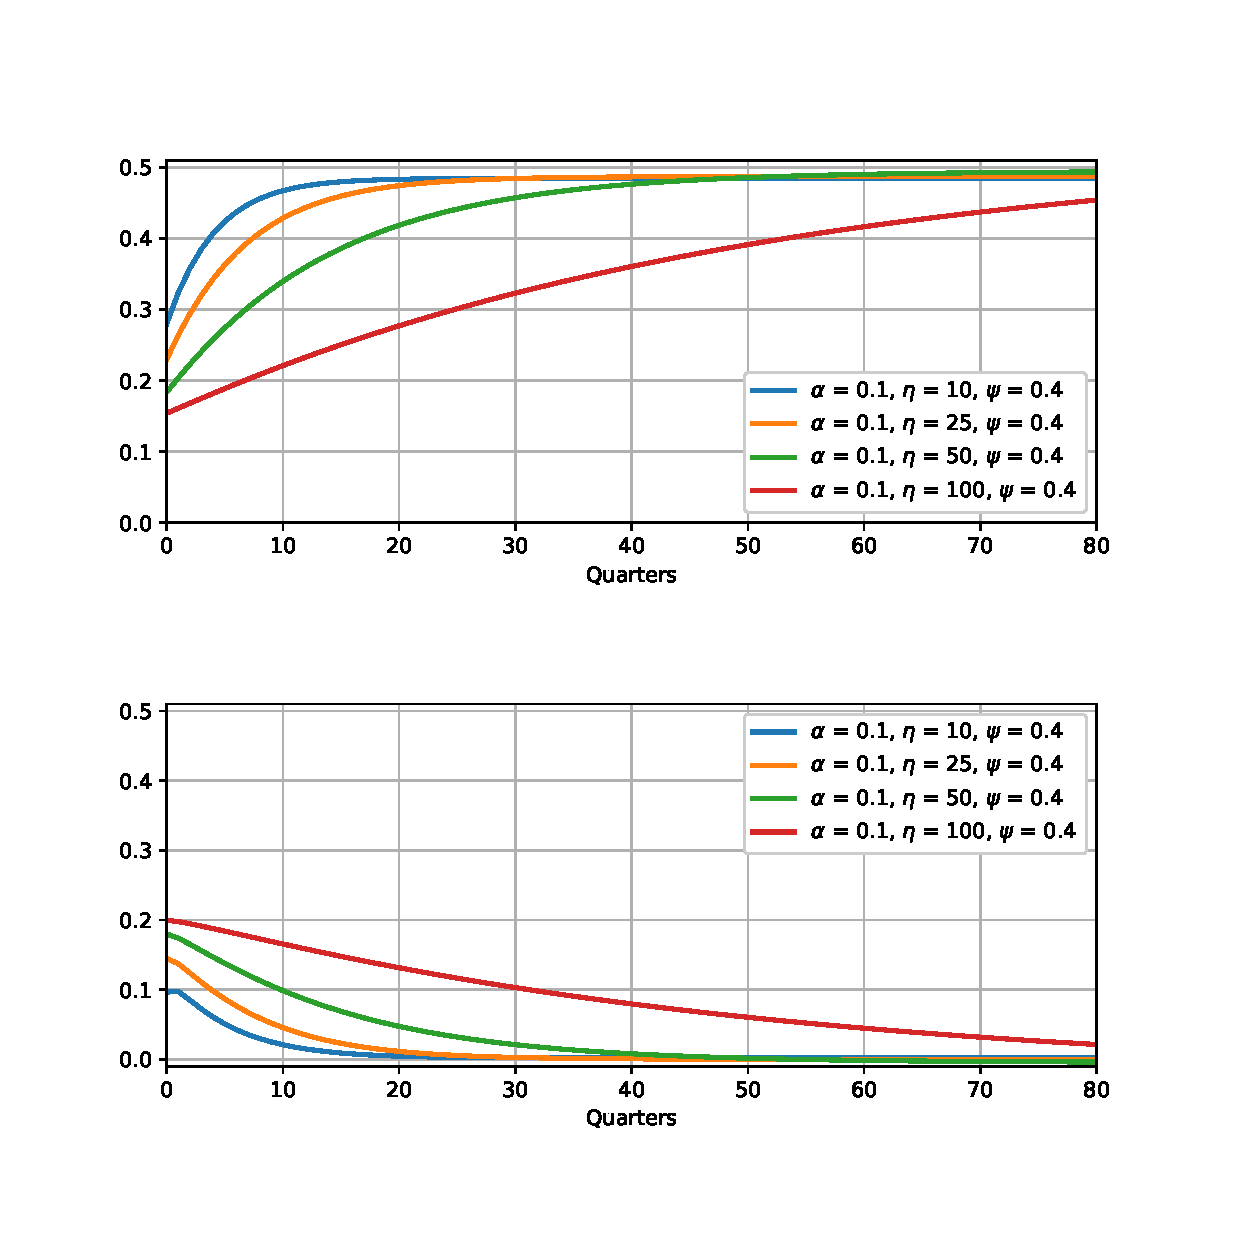
\includegraphics[width=.8\textwidth]{graphs/habit_persistence_impulse_response_varyeta.eps}
\caption{Consumption responses for the two shock processes for habit persistent preferences for $\alpha = .1$, $\psi = .4$ and alternative choice for $\eta$. Top panel: permanent shock.  Bottom panel: transitory shock.  \label{fig:rho_responses}}
\end{figure}

\noindent Figure \ref{fig:alpha_responses} shows how changing $\alpha$ alters the impulse response for the logarithm of consumption for fixed values
$\psi = .4$ and $\eta  = 50$.  While preserving the same qualitative response patterns for consumption, increasing $\alpha$ from $.3$ to $.7$ has little impact on consumption.  At the more extreme $\alpha = .1$ and $.9$ there is substantially more curvature in the initial part of the responses and convergence occurs faster.

\begin{figure}[H]
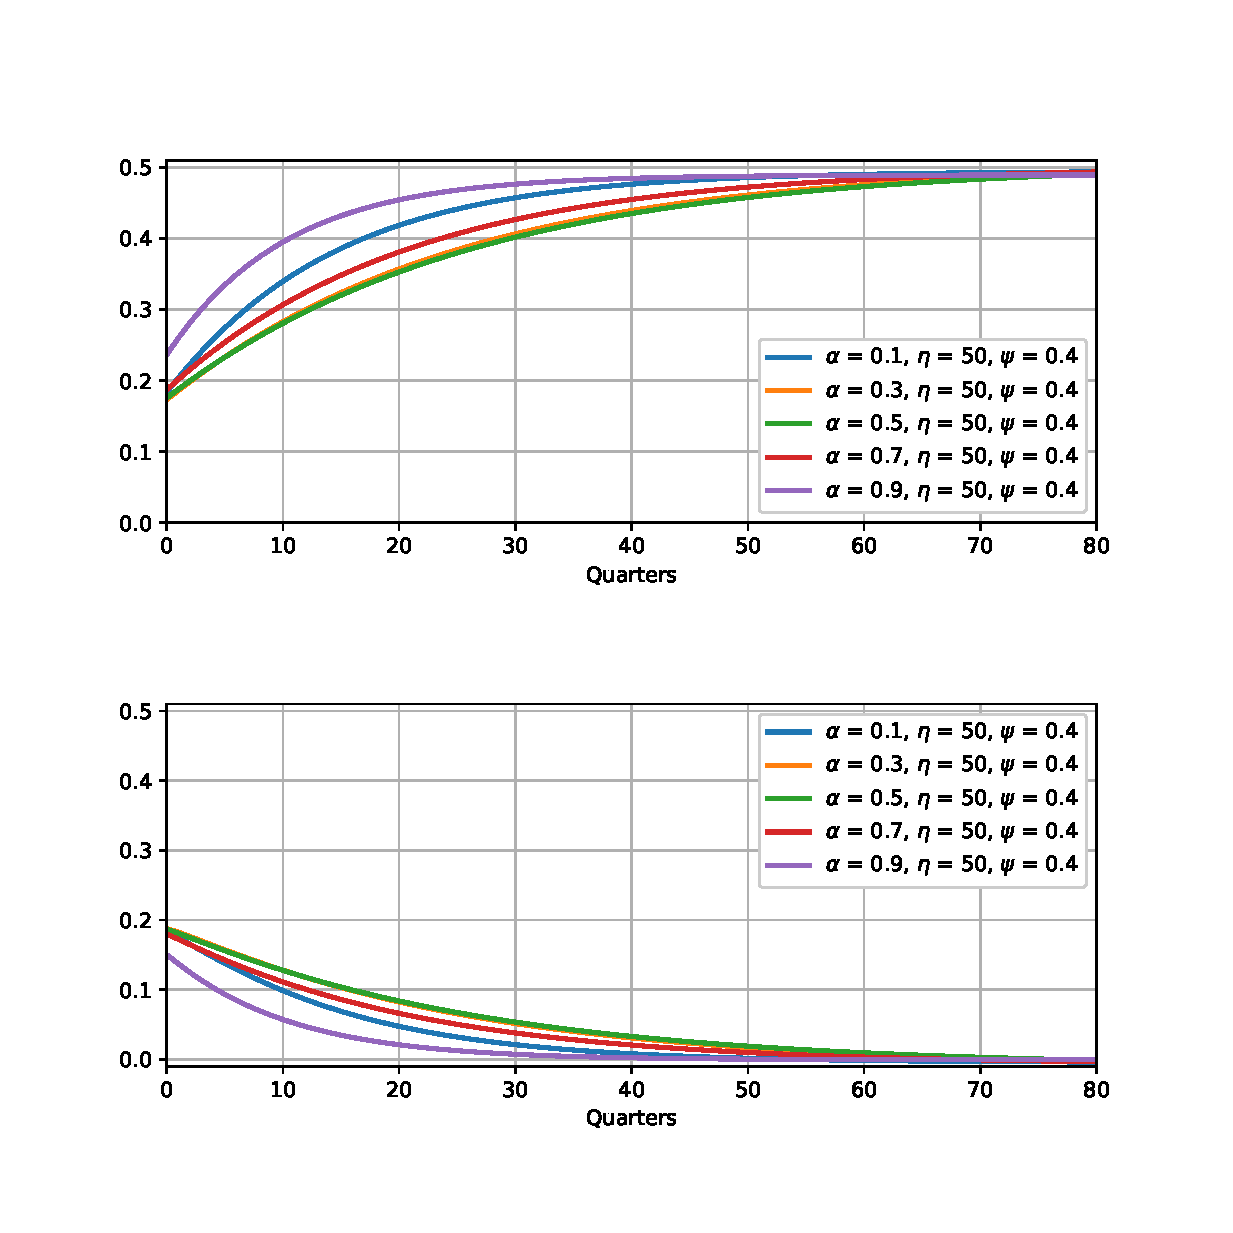
\includegraphics[width=.8\textwidth]{graphs/habit_persistence_impulse_response_varyalpha.eps}
\caption{Consumption responses for the two shock processes for habit persistent preferences for $\eta =  50$, $\psi = .4$ and alternative choice for $\alpha$. Top panel: permanent shock.  Bottom panel: transitory shock.   }\label{fig:alpha_responses}
\end{figure}

\begin{figure}[H]
\includegraphics[width=.8\textwidth]{graphs/habit_persistence_impulse_response_varypsi.eps}
\caption{Consumption responses for the two shock processes for habit persistent preferences for $\alpha = .1$, $\eta =  100$, $\psi = .4, .8,1.6, 2.4$. Top panel: permanent shock.  Bottom panel: transitory shock.  }\label{fig:psi_responses}
\end{figure}

Figure \ref{fig:psi_responses} shows how the consumption impulse response changes when we alter the rate of depreciation  $\psi$ of  household capital. We are particularly interested in the responses to the permanent shock.  As expected,  the responses approximate their limiting value more quickly when we increase $\psi$.  \textcolor{blue}{Lars XXXXX:  could the scale on the $y$ (coordinate) axis in the lower panel be improved to facilitate comparison?} {\color{red} Tom Notice the similarity to the long-run risk consumption response except here we generate endogenously.}









Next we add in a concern about robustness as in \cite{hst:1999}.  This requires that we compute the first-order term for the continuation value process.
\[
V_t = [1 - \exp(-\delta)]  (U_t + Y_t)   - \exp(-\delta)  \xi \log E\left[ \exp \left( - {\frac 1 \xi} V_{t+1} \right) \vert {\mathcal F}_t \right]
\]
Thus
\[
V_t^1 - Y_t^1  =  [1 - \exp(-\delta)] U_t^1  - \exp(-\delta) \xi \log E\left[ \exp \left( - {\frac 1 \xi} V_{t+1}^1 - Y_{t}^1  \right) \vert {\mathcal F}_t \right]
\]
Represent:
\begin{align*}
Y_{t+1}^1 - Y_t^1 & = {\mathbb S}_y \cdot X_t + {\mathbb F}_y \cdot W_{t+1} \cr
U_t^1  & = {\mathbb S}_u \cdot  \begin{bmatrix}  K_{t}^1 \cr H_{t}^1  \cr X_{t} \end{bmatrix} \cr
V_t^1 - Y_t^1 & = {\mathbb S}_v \cdot \begin{bmatrix}  K_{t}^1 \cr H_{t}^1  \cr X_{t} \end{bmatrix} + {\sf s}_v
\end{align*}
where ${\mathbb S}_u$ comes from the model solution using formula \eqref{firstorderutil} and ${\mathbb S}_v$ and ${\sf s}_v$ are to be computed as in \cite{hhl:2008}.  In particular,
\[
({\mathbb S}_v)' =  [1 - \exp(-\delta)] ({\mathbb S}_u)' +   \exp(-\delta) \left[ ({\mathbb S}_v)'  {\mathbb A}  + \begin{bmatrix} 0 & 0 & ({\mathbb S}_y)' \end{bmatrix} \right],
\]
and
\[
{\sf s}_v = \exp(-\delta) \left[ {\sf s}_v - {\frac \xi 2} \left \vert  ({\mathbb S}_v)' {\mathbb B} + ({\mathbb S}_y)' {\mathbb B}_x  \right \vert^2 \right]
\]
The first equation is affine in ${\mathbb S}_v$ and can be solved prior to the second equation.  Given ${\mathbb S}_v$, the second equation is affine in ${\sf v}$ and may be solved easily as well.  We compute uncertainty prices given by the two-dimensional vector:
\[
{\frac 1 \xi} \left[ ({\mathbb S}_v)'{\mathbb B}  + F_y \right] = {\frac 1 \xi} \begin{bmatrix} .482 \cr .00394 \end{bmatrix}
\]
for $(\alpha, \eta, \psi) = (.1, 100, 1.6)$.




%\subsubsection{Inserted comments to LPH}
%
%\textcolor{red}{Lars: might an alternative approach to the computations that you describe in the next subsection  be possible and/or worthwhile?  It would work as follows:
%\begin{itemize}
%\item Reverse engineer a discounted  linear quadratic problem whose first-order conditions are the stacked first-order difference system of  state-costate variables that you are solving in the next section.
%\item Modify this problem to include robustness in standard LQ fashion and get one of the several versions of the Riccati equations in
%\citet{HSrobustnessmonograph}.
%\item Use the Riccati equation and standard formulas that express the matrix factorization that you want in the next section as functions of  the gradient of the value function.
%\end{itemize}
%}

\newpage

\bibliography{knightbib}













\end{document}
